\documentclass[]{article}
\usepackage{lmodern}
\usepackage{amssymb,amsmath}
\usepackage{ifxetex,ifluatex}
\usepackage{fixltx2e} % provides \textsubscript
\ifnum 0\ifxetex 1\fi\ifluatex 1\fi=0 % if pdftex
  \usepackage[T1]{fontenc}
  \usepackage[utf8]{inputenc}
\else % if luatex or xelatex
  \ifxetex
    \usepackage{mathspec}
  \else
    \usepackage{fontspec}
  \fi
  \defaultfontfeatures{Ligatures=TeX,Scale=MatchLowercase}
\fi
% use upquote if available, for straight quotes in verbatim environments
\IfFileExists{upquote.sty}{\usepackage{upquote}}{}
% use microtype if available
\IfFileExists{microtype.sty}{%
\usepackage{microtype}
\UseMicrotypeSet[protrusion]{basicmath} % disable protrusion for tt fonts
}{}
\usepackage[margin=1in]{geometry}
\usepackage{hyperref}
\hypersetup{unicode=true,
            pdftitle={BDA3 Exercises: 1},
            pdfauthor={Oscar Oelrich},
            pdfborder={0 0 0},
            breaklinks=true}
\urlstyle{same}  % don't use monospace font for urls
\usepackage{color}
\usepackage{fancyvrb}
\newcommand{\VerbBar}{|}
\newcommand{\VERB}{\Verb[commandchars=\\\{\}]}
\DefineVerbatimEnvironment{Highlighting}{Verbatim}{commandchars=\\\{\}}
% Add ',fontsize=\small' for more characters per line
\usepackage{framed}
\definecolor{shadecolor}{RGB}{248,248,248}
\newenvironment{Shaded}{\begin{snugshade}}{\end{snugshade}}
\newcommand{\KeywordTok}[1]{\textcolor[rgb]{0.13,0.29,0.53}{\textbf{#1}}}
\newcommand{\DataTypeTok}[1]{\textcolor[rgb]{0.13,0.29,0.53}{#1}}
\newcommand{\DecValTok}[1]{\textcolor[rgb]{0.00,0.00,0.81}{#1}}
\newcommand{\BaseNTok}[1]{\textcolor[rgb]{0.00,0.00,0.81}{#1}}
\newcommand{\FloatTok}[1]{\textcolor[rgb]{0.00,0.00,0.81}{#1}}
\newcommand{\ConstantTok}[1]{\textcolor[rgb]{0.00,0.00,0.00}{#1}}
\newcommand{\CharTok}[1]{\textcolor[rgb]{0.31,0.60,0.02}{#1}}
\newcommand{\SpecialCharTok}[1]{\textcolor[rgb]{0.00,0.00,0.00}{#1}}
\newcommand{\StringTok}[1]{\textcolor[rgb]{0.31,0.60,0.02}{#1}}
\newcommand{\VerbatimStringTok}[1]{\textcolor[rgb]{0.31,0.60,0.02}{#1}}
\newcommand{\SpecialStringTok}[1]{\textcolor[rgb]{0.31,0.60,0.02}{#1}}
\newcommand{\ImportTok}[1]{#1}
\newcommand{\CommentTok}[1]{\textcolor[rgb]{0.56,0.35,0.01}{\textit{#1}}}
\newcommand{\DocumentationTok}[1]{\textcolor[rgb]{0.56,0.35,0.01}{\textbf{\textit{#1}}}}
\newcommand{\AnnotationTok}[1]{\textcolor[rgb]{0.56,0.35,0.01}{\textbf{\textit{#1}}}}
\newcommand{\CommentVarTok}[1]{\textcolor[rgb]{0.56,0.35,0.01}{\textbf{\textit{#1}}}}
\newcommand{\OtherTok}[1]{\textcolor[rgb]{0.56,0.35,0.01}{#1}}
\newcommand{\FunctionTok}[1]{\textcolor[rgb]{0.00,0.00,0.00}{#1}}
\newcommand{\VariableTok}[1]{\textcolor[rgb]{0.00,0.00,0.00}{#1}}
\newcommand{\ControlFlowTok}[1]{\textcolor[rgb]{0.13,0.29,0.53}{\textbf{#1}}}
\newcommand{\OperatorTok}[1]{\textcolor[rgb]{0.81,0.36,0.00}{\textbf{#1}}}
\newcommand{\BuiltInTok}[1]{#1}
\newcommand{\ExtensionTok}[1]{#1}
\newcommand{\PreprocessorTok}[1]{\textcolor[rgb]{0.56,0.35,0.01}{\textit{#1}}}
\newcommand{\AttributeTok}[1]{\textcolor[rgb]{0.77,0.63,0.00}{#1}}
\newcommand{\RegionMarkerTok}[1]{#1}
\newcommand{\InformationTok}[1]{\textcolor[rgb]{0.56,0.35,0.01}{\textbf{\textit{#1}}}}
\newcommand{\WarningTok}[1]{\textcolor[rgb]{0.56,0.35,0.01}{\textbf{\textit{#1}}}}
\newcommand{\AlertTok}[1]{\textcolor[rgb]{0.94,0.16,0.16}{#1}}
\newcommand{\ErrorTok}[1]{\textcolor[rgb]{0.64,0.00,0.00}{\textbf{#1}}}
\newcommand{\NormalTok}[1]{#1}
\usepackage{graphicx,grffile}
\makeatletter
\def\maxwidth{\ifdim\Gin@nat@width>\linewidth\linewidth\else\Gin@nat@width\fi}
\def\maxheight{\ifdim\Gin@nat@height>\textheight\textheight\else\Gin@nat@height\fi}
\makeatother
% Scale images if necessary, so that they will not overflow the page
% margins by default, and it is still possible to overwrite the defaults
% using explicit options in \includegraphics[width, height, ...]{}
\setkeys{Gin}{width=\maxwidth,height=\maxheight,keepaspectratio}
\IfFileExists{parskip.sty}{%
\usepackage{parskip}
}{% else
\setlength{\parindent}{0pt}
\setlength{\parskip}{6pt plus 2pt minus 1pt}
}
\setlength{\emergencystretch}{3em}  % prevent overfull lines
\providecommand{\tightlist}{%
  \setlength{\itemsep}{0pt}\setlength{\parskip}{0pt}}
\setcounter{secnumdepth}{0}
% Redefines (sub)paragraphs to behave more like sections
\ifx\paragraph\undefined\else
\let\oldparagraph\paragraph
\renewcommand{\paragraph}[1]{\oldparagraph{#1}\mbox{}}
\fi
\ifx\subparagraph\undefined\else
\let\oldsubparagraph\subparagraph
\renewcommand{\subparagraph}[1]{\oldsubparagraph{#1}\mbox{}}
\fi

%%% Use protect on footnotes to avoid problems with footnotes in titles
\let\rmarkdownfootnote\footnote%
\def\footnote{\protect\rmarkdownfootnote}

%%% Change title format to be more compact
\usepackage{titling}

% Create subtitle command for use in maketitle
\newcommand{\subtitle}[1]{
  \posttitle{
    \begin{center}\large#1\end{center}
    }
}

\setlength{\droptitle}{-2em}

  \title{BDA3 Exercises: 1}
    \pretitle{\vspace{\droptitle}\centering\huge}
  \posttitle{\par}
    \author{Oscar Oelrich}
    \preauthor{\centering\large\emph}
  \postauthor{\par}
      \predate{\centering\large\emph}
  \postdate{\par}
    \date{11 november 2018}


\begin{document}
\maketitle

Suggested solutions to some of the exercises in Bayesian Data Analysis
3rd edition by Gelman et al.

\section{Chapter 1}\label{chapter-1}

\subsection{Exercise 1.1}\label{exercise-1.1}

\subsubsection{Part a}\label{part-a}

Since \(\theta\) is a discrete variable which takes only the values
\(1\) and \(2\), the marginal probability density for \(y\) will be
obtained by summing over \(\theta\)

\[\begin{equation}
p(y) = \sum_{i=1}^2 p(y|\theta_i) p(\theta_i) = \frac{1}{2}p(y|\theta=1)+\frac{1}{2}p(y|\theta=2)
\end{equation}\] . Using \(\sigma=2\) the density will be given by

\[\begin{equation}
p(y)=\frac{1}{2} \frac{1}{\sqrt{2\pi 2^2}}e^{-(y-1)^2/(2*2^2)}   + \frac{1}{2}\frac{1}{\sqrt{2\pi 2^2}}e^{-(y-2)^2/(2*2^2)}= \frac{1}{4\sqrt{2\pi}}\left(e^{-(y-1)^2/(2*2^2)}+e^{-(y-2)^2/(2*2^2)}\right)
\end{equation}\]

We plot the density

\begin{Shaded}
\begin{Highlighting}[]
\NormalTok{p1 <-}\StringTok{ }\ControlFlowTok{function}\NormalTok{(y) }\FloatTok{0.25}\OperatorTok{*}\NormalTok{(}\DecValTok{1}\OperatorTok{/}\KeywordTok{sqrt}\NormalTok{(}\DecValTok{2}\OperatorTok{*}\NormalTok{pi))}\OperatorTok{*}\NormalTok{(}\KeywordTok{exp}\NormalTok{(}\OperatorTok{-}\NormalTok{(y}\OperatorTok{-}\DecValTok{1}\NormalTok{)}\OperatorTok{^}\DecValTok{2}\OperatorTok{/}\NormalTok{(}\DecValTok{2}\OperatorTok{*}\DecValTok{2}\OperatorTok{^}\DecValTok{2}\NormalTok{))}\OperatorTok{+}\KeywordTok{exp}\NormalTok{(}\OperatorTok{-}\NormalTok{(y}\OperatorTok{-}\DecValTok{2}\NormalTok{)}\OperatorTok{^}\DecValTok{2}\OperatorTok{/}\NormalTok{(}\DecValTok{2}\OperatorTok{*}\DecValTok{2}\OperatorTok{^}\DecValTok{2}\NormalTok{)))}
\CommentTok{# Or we could just use the build in densities from r...}
\CommentTok{#p2 <- function(y) 0.5*dnorm(y, 1, 2)+0.5*dnorm(y,2,2)}
\NormalTok{x <-}\StringTok{ }\KeywordTok{seq}\NormalTok{(}\OperatorTok{-}\DecValTok{5}\NormalTok{, }\DecValTok{8}\NormalTok{, }\FloatTok{0.001}\NormalTok{)}
\KeywordTok{plot}\NormalTok{(x, }\KeywordTok{p1}\NormalTok{(x), }\DataTypeTok{type =} \StringTok{'l'}\NormalTok{)}
\end{Highlighting}
\end{Shaded}

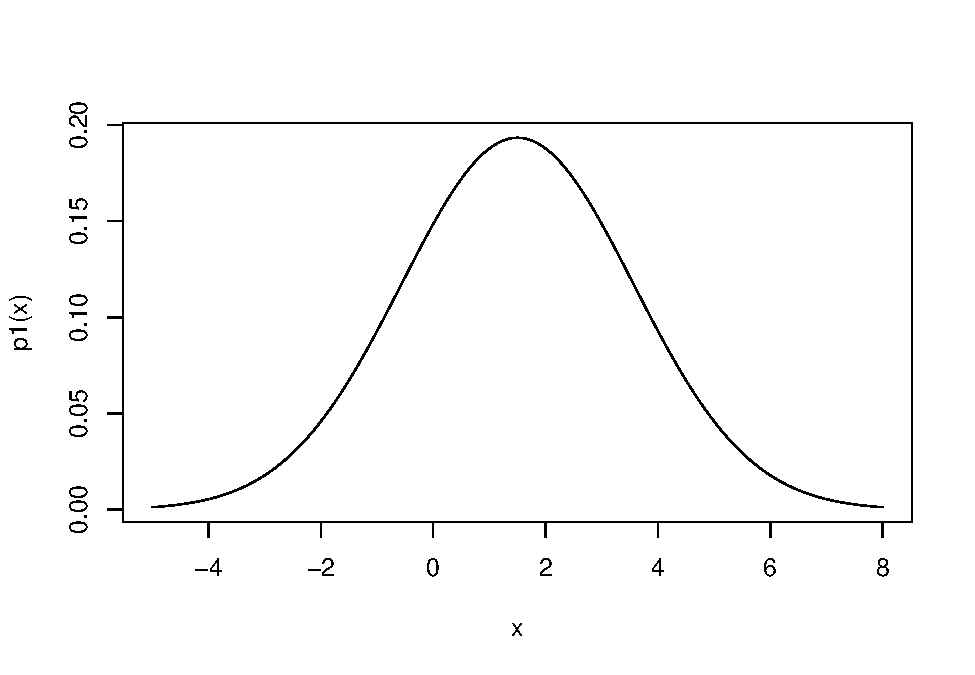
\includegraphics{bda3-exercises-1_files/figure-latex/unnamed-chunk-1-1.pdf}

\subsubsection{Part b}\label{part-b}

Using Bayes' theorem we have that

\[\begin{equation}
p(\theta=1|y=1) = \frac{p(y=1|\theta=1) p(\theta=1)}{p(y=1)}
\end{equation}\]

which we calculate to be

\begin{Shaded}
\begin{Highlighting}[]
\KeywordTok{dnorm}\NormalTok{(}\DecValTok{1}\NormalTok{,}\DecValTok{1}\NormalTok{,}\DecValTok{2}\NormalTok{)}\OperatorTok{*}\FloatTok{0.5}\OperatorTok{/}\NormalTok{(}\FloatTok{0.5}\OperatorTok{*}\KeywordTok{dnorm}\NormalTok{(}\DecValTok{1}\NormalTok{, }\DecValTok{1}\NormalTok{, }\DecValTok{2}\NormalTok{)}\OperatorTok{+}\FloatTok{0.5}\OperatorTok{*}\KeywordTok{dnorm}\NormalTok{(}\DecValTok{1}\NormalTok{,}\DecValTok{2}\NormalTok{,}\DecValTok{2}\NormalTok{))}
\end{Highlighting}
\end{Shaded}

\begin{verbatim}
## [1] 0.5312094
\end{verbatim}

That is, after having observed \(y=1\) we update our believes favouring
\(\theta=1\), but not by much.

\subsubsection{Part c}\label{part-c}

Given that we have observed \(y=1\), decreasing the value of the
variance means that the observation becomes less and less probable under
the alternative \(\theta=2\) and so the posterior will put more and more
weight on \(\theta=1\) as the variance decreases. As the variance
increases, the probabilities under the two values will creep closer to
each other and the posterior will get closer to the prior of
\(\frac{1}{2}\).

\subsection{Exercise 1.2}\label{exercise-1.2}

We wish to show that the following hold when \(u\) is a vector

\[\begin{equation}
\mathbb{E}(u) = \mathbb{E}(\mathbb{E}(u|v))
\end{equation}\]

\[\begin{equation}
\text{var}(u) = \mathbb{E}(\text{var}(u|v))+\text{var}(\mathbb{E}(u|v))
\end{equation}\]

We start with the conditional mean.

\subsection{Exercise 1.6}\label{exercise-1.6}

Approximately \(1/125\) of all births are fraternal twins, and
approximately \(1/300\) of all births are identical twins. Elvis Presley
had a twin brother who died at birth. Given the approximation that half
of all births are boys, what is the probability that Elvis had a twin
brother?

We will solve the problem using Bayes' theorem. We use the following
notation.

\begin{itemize}
\tightlist
\item
  \emph{IT} is the event of an identical twin
\item
  \emph{FT} is the event of a fraternal twin
\item
  \emph{T} denotes the probability of having a twin and is obtained by
  summing \(IT\) and \(FT\)
\item
  \emph{B} denotes the probability of having a brother
\end{itemize}

We then have that

\[\begin{equation}
P((IT)|(T,B))=\frac{P(T,B|(IT))P(IT)}{P(T,B)}
\end{equation}\]

where we have that \(P(T,B|IT)=1\), since if Elvis has an identical
twin, obviously it's a brother, the probability for \(IT\) is given and
the probability
\(P(T,B)=P(IT,B)+P(FT,B)=P(IT)+P(B|FT)P(FT)=1/300+1/2 *1/125\) which
gives the solution

\[\begin{equation}
P((IT)|(T,B))=\frac{1*\frac{1}{300}}{\frac{1}{300}+\frac{1}{2}\frac{1}{125}}=\frac{5}{11}
\end{equation}\]

\subsection{Exerecise 1.7}\label{exerecise-1.7}

In this exercise we will use Bayes theorem to solve the Monty Hall
problem. The key to solving it is in how we chose to condition. Without
loss of generality we call the door we choose \textbf{A}, the door Monty
opens \textbf{B} and the last door (that we can potentially switch to)
door \textbf{C}. We want to calculate the probability of winning when
using the two different strategies available to us (switching and not
switching). Since we picked door \textbf{A}, the probability we are
interested in when we want to find the probability of winning using the
``not switch'' strategy is the probability that the car is behind door
\textbf{A} given that Monty opened door \textbf{B}. We use \(M(-)\) to
denote Monty opening door -, and \(C(-)\) for the car being behind door
-.

\[\begin{equation}
P(C(A)|M(B))=\frac{P(M(B)|C(A))P(C(A))}{P(M(B))}
\end{equation}\]

To calculate this probability we need to calculate the following.

\[\begin{itemize}
\item $P(M(B)|C(A))$, which is the probability that Monty opens door **B** given that the car is behind door **A**. Since the car is behind **A**, Monty can chose between door **B** and **C** freely, and so this probability is $0.5$.
\item The unconditional probability that the car is behind any particular door is $P(C(C))=\frac{1}{3}$
\item The unconditional probability that Monty opens door **B** can be obtained by summing over the conditional probabilities for the car being behind the different doors. If the car is being door **B** it is zero, if the car is behind door **C** it is one and if the car is behind door **A** it is one half, with the probability of the car being behind any particular door being one third for each door, this sums up to one $\frac{1}{2}$.
\end{itemize}\]

Plugging in the values into Bayes theorem we obtain

\[\begin{equation}
P(C(A)|M(B))=\frac{\frac{1}{2}\frac{1}{3}}{\frac{1}{2}}=\frac{1}{3}
\end{equation}\]

If we instead use the ``switching'' strategy, we only need to calculate
one new probability, namely \(P(M(B)|C(C))\), since now we are
interested in \(P(C(C)|M(B))\) (which is the probability of winning by
using the switching strategy, we win if the car is behind the door we
did not chose and that Monty did not open). Given that the car is behind
door \textbf{C}, Monty has no choice but to open door \textbf{B} so this
probability is one. This gives us a chance of winning equal to

\[\begin{equation}
P(C(C)|M(B))=\frac{1\frac{1}{3}}{\frac{1}{2}}=\frac{2}{3}
\end{equation}\]

Note that we could have obtained this by symmetry. Since given that
Monty opens door \textbf{B}, the car is either behind door \textbf{A} or
\textbf{C}. So if we calculate the probability of it being behind
\textbf{A} to be one third, then the probability that it is behind door
\textbf{C} is clearly two thirds.


\end{document}
